\section{A flow-based replacement of the VAE with an invertible \texorpdfstring{$g$}{g}}
\label{sec:flow}

\Cref{sec:arch} compares two ways of instantiating \cref{def:m1,thm:ng} with the VAE-style estimation
machinery of \cite{ng2025}'s Section 4.3 (as implemented, narrower still, in \cref{app:code}). This
section describes a different choice at the same layer of the problem: keep the requirement of
\cref{eq:obs_equiv} and the prior side of the estimation method unchanged, but replace the
stochastic-encoder / decoder / KL machinery of a VAE with a single invertible map -- a normalizing flow.
Nothing here changes \cref{thm:ng}, \cref{as:1,as:2}, or the environment-requirement propositions of
\cref{sec:reqs}; all of those concern the true generative process, not how it is estimated. For the
moment we also set aside the supervised-vs-self-supervised pretraining question of \cref{sec:pretrain}
and assume it is not a concern, exactly as in the discussion that motivates this section;
\cref{sec:flow:summary} notes where that assumption re-enters.

This section keeps two decisions explicitly separate, since conflating them is easy to do and easy to
get wrong: \emph{whether} to require an invertible architecture at all (\cref{sec:flow:motivation,sec:flow:estimation,sec:flow:split,sec:flow:coupling,sec:flow:injective}, all of which are indifferent to
any particular pretrained network), and, only once that is settled, \emph{which concrete pretrained
network} to use (\cref{sec:flow:implementation,sec:flow:recommendation}), and finally what the resulting
training objective actually computes (\cref{sec:flow:objective}).

\subsection{Motivation: an exact fix for the gap in \texorpdfstring{\nameref{sec:archB}}{Option B}}
\label{sec:flow:motivation}
\Cref{sec:ng} requires $g$ to be a $\mathrm{C}^2$ diffeomorphism onto its image. This is what
\nameref{sec:archB} violates: any backbone that reduces dimension -- ResNet-50, an
AutoencoderKL-style network, or any other architecture with a bottleneck -- cannot be injective. This is
not a property of the pretraining objective or of how well the backbone happens to be trained; it is a
dimension-counting fact about any continuous map from a higher-dimensional space to a strictly
lower-dimensional one. \Cref{sec:archB:gap} already makes this point for the specific case of a cached
ResNet-50 embedding; the same argument rules out any other bottleneck backbone equally, regardless of
what produced its weights.

It is not enough to replace the backbone with something injective while keeping separate encoder and
decoder networks. \nameref{sec:archA}'s and \nameref{sec:archB}'s encoder/decoder pairs are both two
independently parameterized networks tied together only by the reconstruction term of the loss; the
decoder is trained to approximate the inverse of the encoder, but nothing forces it to be that inverse
exactly. \Cref{thm:ng} is stated for one map $g$ with an exact inverse, not for a pair of networks that
have merely learned to approximately undo each other. A single invertible network avoids this by
construction: the same parameters define both directions, so encoding and decoding are the forward and
inverse passes of one bijection, with no approximation gap between them.

\subsection{What changes in the estimation method, and what does not}
\label{sec:flow:estimation}
With a VAE, the stochastic posterior $q^{(u)}(\hat Z\mid X)$ (with its own mean/log-variance networks),
the KL term, and the MSE reconstruction term of \cref{app:code} all exist to compensate for not having an
exact inverse: the posterior approximates an intractable true posterior, and the reconstruction term
penalizes the decoder for the cases where it fails to invert the encoder. If $g$ is an exact bijection
(or an injective map with a smooth inverse on its image), none of this machinery is needed. Encoding is
deterministic, $\hat z=f(x)$; reconstruction is exact by construction, $f^{-1}(f(x))=x$ identically; and
training proceeds by exact maximum likelihood via the change-of-variables formula,
\begin{equation}
\log p_X(x) = \log p_{\hat Z}(f(x)) + \log\bigl|\det J_f(x)\bigr|,
\label{eq:flow-nll}
\end{equation}
in place of the ELBO of \cref{app:code}. \Cref{sec:flow:coupling} defines the concrete building block
that will play the role of $f$; \cref{sec:flow:objective} specializes \cref{eq:flow-nll} term by term
once $f$ is fixed to be the BB-plus-head pipeline of \cref{sec:flow:split}.

What does \emph{not} change: the prior side of the estimation method, $p_{\hat Z}(\hat Z)$, is exactly as
in \cref{sec:use} -- the content ANM prior conditioned on $c=(y,t)$, the style prior conditioned on
$r=(t,e)$, the learnable adjacency $\hat A$, the sparsity penalty, and the sink-freezing procedure. All
of that concerns the distribution of $\hat Z$ alone and is indifferent to whether $X$ relates to $\hat Z$
through a VAE or a flow. Only the piece that plays the role of $\hat g$ (and the loss term that goes with
it) is replaced.

\subsection{Splitting the flow into a frozen backbone and a trainable head}
\label{sec:flow:split}
A pretrained invertible backbone (BB) can still be used the way \nameref{sec:archB} uses a frozen
ResNet-50 -- run once, cached, never backpropagated through -- but the result is qualitatively different
from \cref{sec:archB:gap}. The composition of two maps that are each a diffeomorphism onto their image is
itself a diffeomorphism onto its image. So if BB is genuinely injective (or bijective) with a smooth
inverse, and the true mixing $g$ is too (as \cref{def:m1} already assumes), then
$\tilde x=\mathrm{BB}(x)=(\mathrm{BB}\circ g)(Z)$ is not a lossy stand-in for $x$: it is an exact instance
of $\tilde X=\tilde g(Z)$ for the composite map $\tilde g=\mathrm{BB}\circ g$, which is itself a valid
diffeomorphism onto its image. This is exactly the substitution \cref{sec:archB:gap} flags as unexamined
in the ResNet-50 case; here it is closed, provided BB is actually invertible and not merely found to be
informative by the linear probe of \cref{app:probe} (that diagnostic was designed for the lossy case and
asks a weaker question than exact invertibility).

The remaining, trainable piece of the pipeline is a second invertible map, the \textbf{head}, sitting
between BB's output and the latent variable $\hat Z$ that the prior of \cref{sec:use} is defined over.
Unlike BB, the head starts untrained and is fit by the training objective of \cref{sec:flow:objective}.

What is kept from \nameref{sec:archB}: BB's forward pass still runs once per image and can be cached,
with no gradient reaching it, so the iteration-speed argument for splitting the pipeline still applies.

What is lost relative to \nameref{sec:archB}: an injective map cannot reduce dimension (by the same
counting argument as \cref{sec:flow:motivation}, in reverse), so $\tilde x$ is at least as large as $x$,
not a compact $\sim\!3000$-dimensional embedding. The trainable head therefore cannot be the small MLPs
of \cref{app:code} (\texttt{mean\_net}, \texttt{log\_var\_net}); it has to be a genuine flow operating on
a large tensor. \Cref{sec:flow:memory} quantifies the consequence.

\subsection{The coupling-block architecture, and where the Jacobian term comes from}
\label{sec:flow:coupling}
Both BB and the head considered here are built from the same kind of building block -- a
\emph{coupling layer} -- stacked many times, alternating which half of the vector is updated so that
every coordinate is eventually transformed using every other coordinate over enough layers. This
subsection makes precise the additive- and affine-coupling constructions referred to loosely elsewhere in
this section.

\paragraph{Setup and notation.} A network such as i-RevNet never flattens the image: at every layer the
data is kept as a tensor of shape $(C,H,W)$ -- $C$ channels, each an $H\times W$ spatial map (the input's
3 channels are the R, G, B planes; a channel deeper in the network is a learned feature map, e.g.\
responding to some texture or edge orientation, still laid out over the same $H\times W$ grid). At one
coupling layer, the layer's input is such a tensor with $C$ channels and $n=C\cdot H\cdot W$ entries in
total; $x\in\R^n$ below is just this tensor's entries counted as a vector, purely for writing the Jacobian
as a matrix -- the actual computation never reshapes it. The coupling split partitions the $C$ channels
into two disjoint groups, $x_1$ (the first $C_1$ channels, a tensor of shape $(C_1,H,W)$) and $x_2$ (the
remaining $C_2$ channels, shape $(C_2,H,W)$), with $C_1+C_2=C$ and correspondingly $n_1=C_1HW$,
$n_2=C_2HW$, $n_1+n_2=n$; $x_1$ and $x_2$ are two groups of feature channels of the same spatial map, not
separate tensors of different origin. The layer produces an output $y=(y_1,y_2)$ of the same two shapes,
from which $x$ can be recovered exactly.

\paragraph{Additive coupling (NICE, RevNet, i-RevNet).} Let $F:\R^{n_1}\to\R^{n_2}$ be an arbitrary
neural network -- in i-RevNet, a small residual stack of convolution/batch-norm/ReLU layers. Only $F$'s
input and output shapes are fixed by the construction, not its internals: $F$ must take a $(C_1,H,W)$
tensor and return a $(C_2,H,W)$ tensor, matching $x_1$ and $x_2$ exactly, because \cref{eq:additive-coupling}
below adds $F(x_1)$ directly to $x_2$ -- with no internal downsampling or upsampling, since the addition
also requires $F$ to preserve the spatial resolution $H\times W$. Depth, hidden-channel width, and kernel
size inside $F$ are otherwise unconstrained. Crucially, $F$ itself need not be invertible, and in
i-RevNet it is not: an ordinary residual block with ReLU nonlinearities is not one-to-one (negative inputs
are clipped to $0$, among other things), and nothing in what follows requires it to be. The layer
computes
\begin{equation}
y_1=x_1,\qquad y_2=x_2+F(x_1).
\label{eq:additive-coupling}
\end{equation}
This is invertible for \emph{any} $F$ -- invertible or not -- with the inverse obtained by rearranging
\cref{eq:additive-coupling}:
\[
x_1=y_1,\qquad x_2=y_2-F(y_1).
\]
Note that $F$ is evaluated at the same value both ways ($x_1$ forward, $y_1=x_1$ backward), so inverting
the layer only ever runs $F$ forward again; it never asks for $F^{-1}$. This is why the layer's
invertibility does not depend on $F$ being invertible, and why an arbitrarily complicated (and
non-invertible) $F$ costs nothing extra. The Jacobian of \cref{eq:additive-coupling} with respect to
$(x_1,x_2)$ is
\[
J=\begin{pmatrix}
\partial y_1/\partial x_1 & \partial y_1/\partial x_2\\[2pt]
\partial y_2/\partial x_1 & \partial y_2/\partial x_2
\end{pmatrix}
=\begin{pmatrix}
I_{n_1} & 0\\[2pt]
\partial F/\partial x_1 & I_{n_2}
\end{pmatrix},
\]
block lower-triangular with identity blocks on the diagonal, so
\[
\det J=\det(I_{n_1})\cdot\det(I_{n_2})=1,
\]
exactly, regardless of what $F$ computes. Successive layers alternate which half plays the role of $x_1$
versus $x_2$, so that both halves eventually get updated over depth; this does not change the argument,
since each individual layer still has determinant $1$, and the determinant of a composition of layers is
the product of the individual determinants. Hence a whole stack of such layers -- BB, or an all-additive
head -- has $\det J=1$ as well, however many layers deep, with nothing to compute at any point.

\paragraph{Affine coupling (RealNVP, Glow).} The generalization used when a nonzero log-determinant is
wanted adds a learned elementwise \emph{scale}, computed by a second network $s:\R^{n_1}\to\R^{n_2}$,
alongside a translation network $t:\R^{n_1}\to\R^{n_2}$ (which plays the role $F$ played above, and
inherits the same fixed input/output shape and freedom from needing to be invertible):
\begin{equation}
y_1=x_1,\qquad y_2=x_2\odot\exp\bigl(s(x_1)\bigr)+t(x_1),
\label{eq:affine-coupling}
\end{equation}
where $\odot$ denotes elementwise multiplication. As with $F$ above, $s$ and $t$ are only ever evaluated
forward (at $x_1$, or, when inverting, at $y_1$), never inverted themselves; the inverse of
\cref{eq:affine-coupling} is
\[
x_1=y_1,\qquad x_2=\bigl(y_2-t(y_1)\bigr)\odot\exp\bigl(-s(y_1)\bigr).
\]
The Jacobian is again block lower-triangular,
\[
J=\begin{pmatrix}
I_{n_1} & 0\\[2pt]
\partial y_2/\partial x_1 & \mathrm{diag}\bigl(\exp(s(x_1))\bigr)
\end{pmatrix},
\]
so
\[
\det J=\prod_{i=1}^{n_2}\exp\bigl(s(x_1)_i\bigr)=\exp\Bigl(\textstyle\sum_i s(x_1)_i\Bigr),
\]
giving
\begin{equation}
\log\bigl|\det J\bigr| = \sum_{i=1}^{n_2} s(x_1)_i.
\label{eq:affine-logdet}
\end{equation}
This is a plain sum over the $n_2$ entries of $s(x_1)$, a vector already computed as part of the forward
pass that builds $y_2$ -- no separate determinant algorithm, no matrix operation of any kind, just an
$O(n_2)$ reduction; the log-determinant of a stack of such layers is the sum of each layer's own term.

Both constructions have triangular Jacobians, and both are cheap; the difference between them is
representational, not computational. Additive coupling can only shift $x_2$ by $F(x_1)$, so it preserves
volume exactly ($\det J=1$ always, \cref{eq:additive-coupling}); affine coupling can also rescale $x_2$
coordinate-wise via $\exp(s(x_1))$, so it can locally compress or expand volume, at the cost of the one
extra sum of \cref{eq:affine-logdet} per layer.

\begin{remark}[i-RevNet's actual structure is richer than the bare additive-coupling stack above]
\label{rem:irevnet-structure}
The additive-coupling layer of \cref{eq:additive-coupling} is the building block i-RevNet stacks, but
\cite{jacobsen2018}'s own construction wraps a few further exactly-invertible operators around it that the
simplified picture above elides. At the two ends of the network, one-time split and merge operators
$\tilde{\mathcal S}/\tilde{\mathcal S}^+$ and $\tilde{\mathcal M}/\tilde{\mathcal M}^{-1}$ move data between
the image's channel layout and the two coupling streams (and back, at the output); like the coupling split
above, these are fixed, invertible bookkeeping, not something learned in the sense $F$ is. More importantly,
at each stage $j$ the stream that is \emph{not} passed through the residual function -- called $\mathcal
S_j$ in \cite{jacobsen2018} -- is not simply carried forward unchanged as $y_1=x_1$ in \cref{eq:additive-coupling}: it has its own explicit, stated inverse $\mathcal S_j^{-1}$, unlike the residual function
$F_j$, which (as noted above) is never inverted and need not be invertible at all. An operator with a
non-trivial stated inverse is exactly the kind of map that can have a non-identity Jacobian block on that
stream -- for instance a per-channel rescaling or a fixed permutation/downsampling reshuffle -- in which
case it contributes its own diagonal log-determinant term, of the same $O(n_2)$-sum form as
\cref{eq:affine-logdet}, alongside the coupling layers' own terms, rather than the two streams' Jacobian
blocks both being identity as the bare-NICE picture above assumes. The $\mathcal S_j$ in the specific
i-RevNet variant used in
the released architecture/checkpoint is analyzed in \cref{app:irevnet:jacobian}.

\begin{figure}[H]
\centering
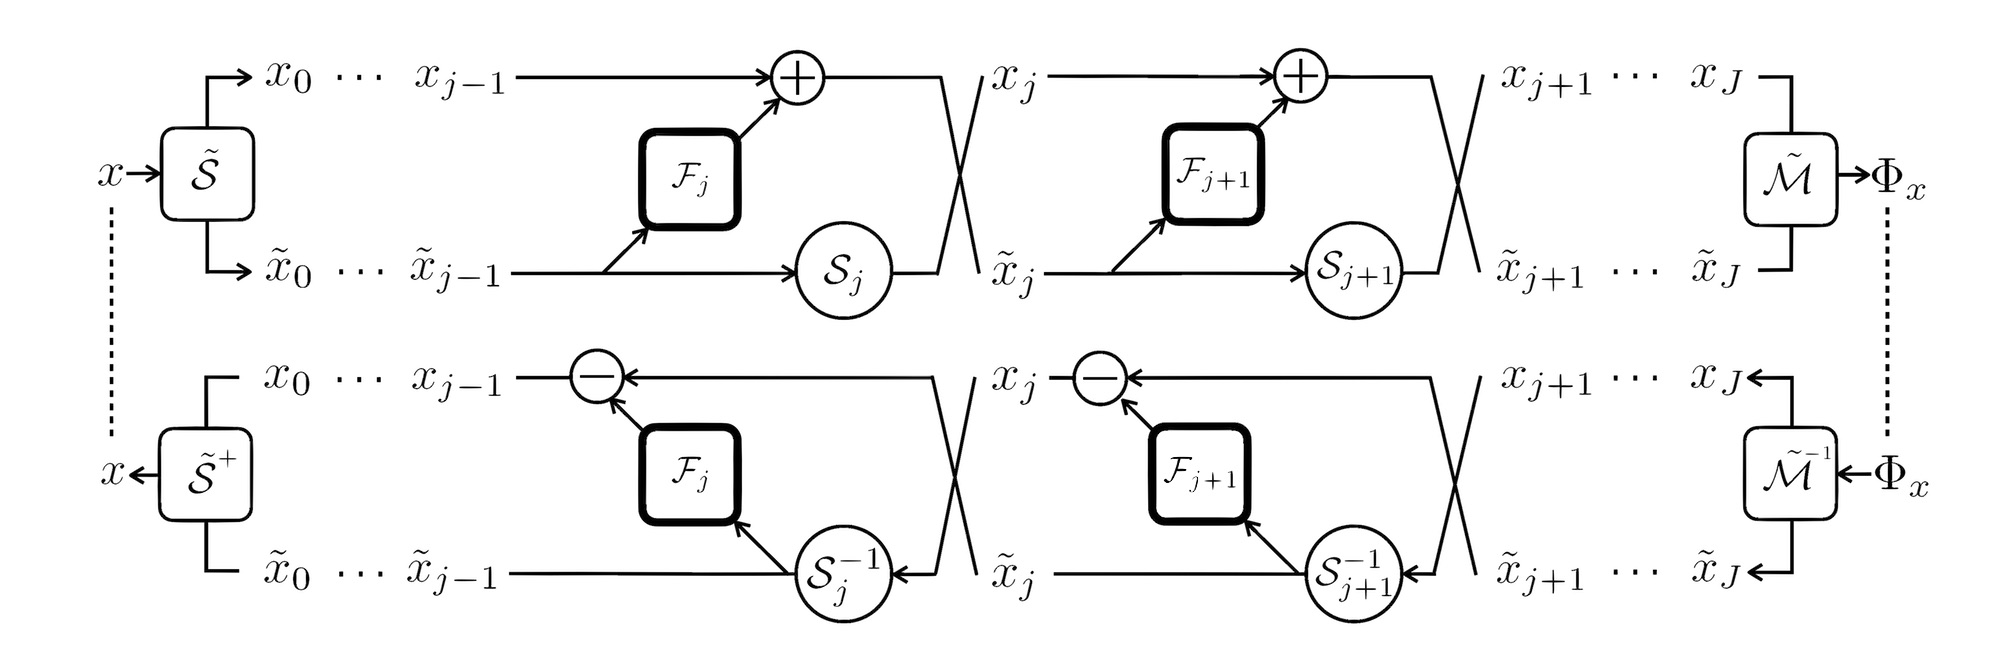
\includegraphics[width=0.95\textwidth]{irevnet-algorithm.jpg}
\caption{The i-RevNet building block, reproduced from \cite{jacobsen2018} (forward pass, top row; inverse,
bottom row). $\tilde{\mathcal S}/\tilde{\mathcal S}^+$ and $\tilde{\mathcal M}/\tilde{\mathcal M}^{-1}$ are
the one-time split/merge operators at the two ends; $\mathcal F_j$ is the (non-invertible, never-inverted)
residual function of \cref{eq:additive-coupling}'s $F$; $\mathcal S_j$ acts on the stream that is not passed
through $\mathcal F_j$ at stage $j$, with its own stated inverse $\mathcal S_j^{-1}$ used on the inverse
path (bottom row). \textbf{What the crossing between consecutive stages means:} at stage $j$ the top stream
$x_{j-1}$ is combined with $\mathcal F_j(\tilde x_{j-1})$ at the $\oplus$ node (this is $y_2=x_2+F(x_1)$ of
\cref{eq:additive-coupling}, with the bottom stream playing $x_1$), while the bottom stream is itself
mapped through $\mathcal S_j$ rather than carried forward unchanged; the crossing lines immediately after
then swap these two results before stage $j+1$, so that the just-updated ($\oplus$-node) stream becomes the
input fed into $\mathcal F_{j+1}$ next, and the $\mathcal S_j$-transformed stream becomes the one updated at
the next $\oplus$. This is the diagrammatic realization of the alternation already described in the main
text above (``successive layers alternate which half plays the role of $x_1$ versus $x_2$''); the only
difference from the bare picture given there is that the carried-forward stream is passed through $\mathcal
S_j$ at each stage rather than left as the identity, which is the source of the possible extra log-det term
this remark flags.}
\label{fig:irevnet-algorithm}
\end{figure}
\end{remark}

\subsection{Injective versus bijective: what the theorem requires, and what each costs to compute}
\label{sec:flow:injective}
Everything so far applies to \emph{any} invertible BB; this subsection is the last purely architectural
one before \cref{sec:flow:implementation} asks which concrete network to use.

\Cref{sec:ng} asks only that $g$ be a diffeomorphism \emph{onto its image}; it does not require the
output dimension to equal the input dimension. An injective embedding into a strictly larger space
satisfies this exactly as well as a dimension-preserving bijection does. Both options require output
dimension at least as large as input dimension -- a bijection meets this with equality, an injective
embedding sits above it -- and this floor is unavoidable for any exactly invertible map; it is not a
special cost of choosing the injective option over the bijective one.

There is, however, a real and separate cost that does distinguish the two, on the computational side of
\cref{eq:flow-nll}. \Cref{sec:flow:coupling} shows that a square (dimension-preserving) map built from
either coupling construction has a triangular Jacobian and is cheap to evaluate -- exactly free
($\det J=1$) for additive coupling regardless of depth \cite{gomez2017}, an $O(n)$ sum for affine
coupling. For a genuinely injective (non-square, dimension-expanding) map, neither of these
constructions, nor the triangular argument behind them, applies: with no square Jacobian, the correct
change-of-volume term is instead the Jacobian-transpose-Jacobian determinant $\det(J^\top J)^{1/2}$ (a
Gram determinant), and computing this -- or even a usable gradient of it -- is a substantially harder
problem that is the subject of ongoing, unresolved research (\emph{Rectangular Flows}, \cite{caterini2021});
current approaches either approximate the term or avoid computing it at all. This is not a limitation of
one particular network; it is a property of dimension-expanding invertible maps in general.

So the dimension-preserving, bijective option is preferable on two independent grounds, not one: it does
not buy accuracy the M1 use case does not need (a point returned to in \cref{sec:flow:implementation}),
and its Jacobian term in \cref{eq:flow-nll} is cheap or free by construction, where the injective
alternative's is an open computational problem. The remainder of this section assumes a bijective,
dimension-preserving BB.

\subsection{Choosing an implementation: i-RevNet versus generative normalizing flows}
\label{sec:flow:implementation}
With ``bijective, coupling-based invertible network'' settled as the architecture family, a separate
question remains: which concrete, ideally pretrained, network to actually use. Three properties matter,
and no candidate available today satisfies all three at once.
\begin{enumerate}[label=(\roman*),leftmargin=2.2em]
\item \label{item:inv} \textbf{Genuinely invertible from raw pixels}, i.e.\ no lossy step anywhere
      between $x$ and the representation used downstream.
\item \label{item:res} \textbf{Pretrained at the target resolution and scale} (full $224\times224$
      general-purpose images, not a narrow domain or a heavily downsampled variant).
\item \label{item:obj} \textbf{Pretrained by an objective aligned with \cref{eq:obs_equiv}}, i.e.\
      density/maximum-likelihood estimation, rather than by a discriminative objective unrelated to
      matching a distribution.
\end{enumerate}

\paragraph{i-RevNet (classification-pretrained).} \cite{jacobsen2018} is a stack of exactly the additive
coupling blocks of \cref{eq:additive-coupling}, pretrained on ImageNet with the standard supervised
classification objective, in a dimension-preserving bijective variant ($\sim$29M parameters, 26.7\%
top-1 error) and a channel-widening injective variant ($\sim$181M parameters, 24.7\% top-1 error,
matching a same-size ResNet-50); \cref{sec:flow:injective}'s argument already favors the bijective one.
It satisfies \labelcref{item:inv} exactly and \labelcref{item:res} directly -- a public, full-resolution
ImageNet-1k checkpoint. It fails \labelcref{item:obj}: nothing in cross-entropy training targets
density estimation. But, per \cref{sec:flow:coupling,sec:flow:injective}, this failure is cheap to have:
because the Jacobian of an additive-coupling block is exactly $1$ regardless of what the block was
trained to do, a classification objective does not make \cref{eq:flow-nll} harder or more expensive to
evaluate -- it can only affect the \emph{geometry} of the learned representation (how conveniently the
surviving, fully-preserved information is arranged for the downstream head and prior to work with), not
whether that information survived (guaranteed by invertibility) or how expensive it is to use.

\paragraph{Off-the-shelf generative normalizing flows (Glow, RealNVP, Residual Flows, \dots).} These are
trained by exact maximum likelihood, so they satisfy \labelcref{item:obj} squarely, and their
square, coupling/1x1-convolution-based architecture satisfies \labelcref{item:inv}. They fail
\labelcref{item:res}: every publicly released checkpoint for this family is at ImageNet $32\times32$ or
$64\times64$ (downsampled) or at CelebA-HQ ($256\times256$, but faces, a much narrower domain), never at
full-resolution general ImageNet. Using one here means retraining from that resolution upward, which
gives up most of what ``pretrained'' was supposed to buy.

\paragraph{Modern large-scale flows (e.g.\ STARFlow \cite{gu2025starflow}).} Recent work has scaled
normalizing flows to real image resolutions with public checkpoints, which looks at first like a
resolution of \labelcref{item:res} for a genuine density-estimation objective. It is not a resolution of
\labelcref{item:inv}, however: this line of work achieves scale specifically by placing the flow inside
the latent space of a standard, lossy autoencoder (an AutoencoderKL-style network) rather than by making
the pixel-to-representation map itself invertible. Adopting it here would reopen exactly the gap
\cref{sec:archB:gap} and \cref{sec:flow:motivation} exist to close, not close it -- the pixel-to-latent
step is the same kind of bottleneck as ResNet-50, only wrapped in a flow further downstream.

\paragraph{Training a bijective coupling flow from scratch on TerraInc-scale data.} The only option that
can satisfy \labelcref{item:inv,item:res,item:obj} simultaneously, since it is fit directly to the target
data and resolution by maximum likelihood, with an architecture chosen for exact invertibility from the
start. The cost is that it gets no benefit from pretraining at all; in that respect it is closer in
spirit to \nameref{sec:archA} (train everything, pay the full cost) than to the frozen-backbone split
this section otherwise describes.

\subsection{Recommendation}
\label{sec:flow:recommendation}
No currently available pretrained network satisfies all three criteria of \cref{sec:flow:implementation}
at once, so the choice is between which criterion to give up. i-RevNet's bijective variant is the
recommended starting point: it is the only candidate that is simultaneously invertible from raw pixels
and available pretrained at the target resolution, and \cref{sec:flow:injective,sec:flow:implementation}
together show that the criterion it fails -- a density-estimation pretraining objective -- is, for this
specific architecture family, a representation-geometry concern rather than a computational one: the
Jacobian term is exactly as cheap under classification pretraining as it would be under any other
objective. That concern is not left untested: it is precisely what the calibration loop already described
in \cref{sec:flow:depth} (held-out negative log-likelihood, plus a separability version of the
linear-probe diagnostic of \cref{app:probe}) is designed to catch. If that calibration shows the
classification-pretrained representation is a poor starting point for the content/style prior to work
with, the fallback is training a bijective coupling flow from scratch (the last option of
\cref{sec:flow:implementation}) -- for the head alone, or, if needed, in place of a pretrained BB
entirely.

\subsection{The training objective, term by term}
\label{sec:flow:objective}
Fixing BB to be the pretrained, frozen i-RevNet bijective backbone of \cref{sec:flow:recommendation}, and
the head to be a second, untrained network built from the coupling-block family of \cref{sec:flow:coupling}
(to be learned from data), the estimation step for one image $x$ from environment $u=(y,t,e)$ proceeds as
follows, replacing \texttt{Trainer.step} of \cref{app:code} term by term.

\begin{enumerate}[label=(\arabic*),leftmargin=2em]
\item \textbf{Encode, deterministically.} Compute $\tilde x=\mathrm{BB}(x)$ (frozen; can be cached once,
      as in \nameref{sec:archB}), then $\hat z=\mathrm{head}^{-1}(\tilde x)$. There is no sampling and no
      \texttt{mu}/\texttt{logvar}: $\hat z$ is one specific value for each $x$.
\item \textbf{Evaluate the prior at $\hat z$, not a KL divergence.} Splitting $\hat z$ into content and
      style blocks as in \cref{eq:split}, compute
      \begin{quote}
      \texttt{cond\_mean=mean\_net(adj\_mat*hat\_z\_c)} and \\
      \texttt{prior\_log\_var=log\_var\_net(domain\_embedding(u))}
      \end{quote}
      exactly as \cref{app:code} already does, and evaluate the ANM/style log-density at the single point
      $\hat z$:
      \begin{equation}
      \log p_{\hat Z}(\hat z\mid u) = \log p\bigl(\hat z_c\bigm|\texttt{cond\_mean},\texttt{prior\_log\_var}\bigr)
      + \sum_{j=1}^{n_s}\log p^{(r)}(\hat z_{s,j}).
      \label{eq:flow-prior-term}
      \end{equation}
      This is the same \texttt{Normal.log\_pdf} computation \cref{app:code} already implements; the only
      change is that it is evaluated once, at a deterministic $\hat z$, rather than compared against an
      approximate posterior.
\item \textbf{Add the encoding map's Jacobian term, via the chain rule.} Writing
      $\Phi=\mathrm{head}^{-1}\circ\mathrm{BB}$ for the full map $x\mapsto\hat z$, the inverse function
      theorem applied to $\mathrm{head}$ gives
      \begin{equation}
      \log\bigl|\det J_\Phi(x)\bigr| = \log\bigl|\det J_{\mathrm{BB}}(x)\bigr|
      - \log\bigl|\det J_{\mathrm{head}}(\hat z)\bigr|.
      \label{eq:flow-jac-split}
      \end{equation}
      Per \cref{sec:flow:coupling,sec:flow:injective}, $\log|\det J_{\mathrm{BB}}(x)|=0$ exactly, since BB
      is built from additive coupling (\cref{eq:additive-coupling}); this term is omitted from the code
      entirely, not computed and found to be zero. $\log|\det J_{\mathrm{head}}(\hat z)|$ is likewise
      exactly $0$ if the head is also pure additive coupling, or the sum of \cref{eq:affine-logdet} over
      the head's constituent layers if the head uses affine coupling instead.
\item \textbf{Assemble the loss.} Combining \cref{eq:flow-nll,eq:flow-prior-term,eq:flow-jac-split} with
      the sparsity penalty of \cref{app:code},
      \begin{equation}
      \mathcal L(x,u) = -\log p_{\hat Z}(\hat z\mid u) - \log\bigl|\det J_{\mathrm{BB}}(x)\bigr|
      + \log\bigl|\det J_{\mathrm{head}}(\hat z)\bigr| + \lambda_{\mathrm{sparse}}\,\ell_{\mathrm{sparse}}(\hat A),
      \label{eq:flow-loss}
      \end{equation}
      where $\ell_{\mathrm{sparse}}(\hat A)$ is \texttt{loss\_sparsity} of \cref{app:code}, computed from
      \texttt{current\_adj\_mat} exactly as before.
\end{enumerate}
\Cref{eq:flow-loss} replaces \texttt{loss\_kl}, \texttt{loss\_rec}, and their weights
\texttt{lambda\_kl}, \texttt{lambda\_rec} outright; \texttt{loss\_sparsity} and \texttt{lambda\_sparse}
carry over unchanged, as does every part of \cref{sec:use}'s prior machinery
(\texttt{mean\_net}, \texttt{log\_var\_net}, \texttt{domain\_embedding}, \texttt{ADJMatrix},
\texttt{find\_sinknodes\_and\_fix}), none of which is aware of, or affected by, how $\hat z$ was produced.

\paragraph{The special case of a purely additive head.} If the head, like BB, uses only additive coupling,
both Jacobian terms of step (3) vanish identically and \cref{eq:flow-loss} reduces to
\begin{equation}
\mathcal L(x,u) = -\log p_{\hat Z}(\hat z\mid u) + \lambda_{\mathrm{sparse}}\,\ell_{\mathrm{sparse}}(\hat A),
\label{eq:flow-loss-additive}
\end{equation}
with no Jacobian computation anywhere in the pipeline: the objective is simply to maximize the prior's
log-density at the transformed point, plus the sparsity penalty -- the same simplification that made the
original NICE construction tractable. The cost is architectural, not computational: a composition of
purely additive-coupling maps can only permute/rearrange density, never locally compress or expand it
(\cref{sec:flow:coupling}), so all of the actual density-shaping needed to match $p_X^{(u)}(x)$ has to
come from the prior side ($\hat A$, \texttt{mean\_net}, \texttt{log\_var\_net}) rather than from $g$
itself. This is not a violation of \cref{thm:ng} -- the theorem only requires \emph{some} diffeomorphism,
and volume-preserving is a valid special case -- but it is a genuine constraint on how flexibly the model
can ultimately fit the observed distribution. If this constraint turns out to bind in practice, the head
(never BB, which is fixed and pretrained) can be switched from additive to affine coupling
(\cref{eq:affine-coupling}), reintroducing the cheap $O(n)$ sum of \cref{eq:affine-logdet} in exchange for
the head being able to locally rescale density rather than merely permute it. \Cref{sec:flow:depth}'s
calibration loop, using held-out $\mathcal L$ from \cref{eq:flow-loss} or \cref{eq:flow-loss-additive} as
appropriate, is the natural place to check whether this constraint is actually binding before paying for
affine coupling. \Cref{sec:flow:headarch} below settles this concretely: for the reasons given there,
affine coupling (not the purely additive case just described) is taken as the default for head, not a
fallback reached for only if a later diagnostic demands it.

\subsection{Head architecture: departing from BB's coupling family}
\label{sec:flow:headarch}
\Cref{sec:flow:split} leaves head's own architecture unspecified beyond ``a genuine flow operating on a
large tensor.'' This subsection fixes it concretely, building on the coupling-layer machinery of
\cref{sec:flow:coupling} but not reusing BB's own block design, for reasons given below.

\paragraph{Head's fixed input/output shape.} The bijective i-RevNet checkpoint of
\cref{sec:flow:recommendation}\footnote{Config \texttt{nBlocks=[6,16,72,6]}, \texttt{nStrides=[2,2,2,2]},
\texttt{nChannels=[24,96,384,1536]}, \texttt{init\_ds=2}, as released for the pretrained model on
\cite{jacobsen2018}'s repository; \texttt{nChannels} denotes channels per coupling stream, not the total.}
applies five factor-2 invertible-squeeze downsamplings in total (\texttt{init\_ds=2} plus the four stage
strides), each quadrupling channels while halving each spatial dimension, taking $3\times224\times224$ to
two streams of $1536$ channels at $7\times7$, i.e.\ a total of $C=3072$ channels at $H=W=7$. As a check,
$C\cdot H\cdot W=3072\cdot49=150528=3\cdot224\cdot224$: exactly the input pixel count, confirming BB is
dimension-preserving as \cref{sec:flow:recommendation} requires. Head therefore never sees a raw image;
its input and output are both this fixed $3072\times7\times7$ tensor, and -- unlike BB -- head needs no
further spatial squeeze stages, since the spatial dimension is already collapsed to $7\times7$: its whole
depth budget goes into channel-mixing and coupling blocks at this one fixed resolution.

\paragraph{Why head should not copy either of BB's own configurations (additive, i-RevNet-style).}
Per \cref{sec:flow:coupling}, additive coupling has $\det J=1$ exactly, so a stack of purely
additive-coupling layers can only permute/rearrange density, never reshape it
(\cref{eq:flow-loss-additive}'s discussion above). BB is fixed to additive coupling, so if head is
\emph{also} purely additive, \emph{no} part of the learned map $g=\mathrm{head}\circ\mathrm{BB}$ can locally
compress or expand volume anywhere; all of the density-shaping needed to match $p_X^{(u)}(x)$ would have to
come entirely from the prior side ($\hat A$, \texttt{mean\_net}, \texttt{log\_var\_net}). Since head is the
only trainable piece of $g$, it should default to affine coupling (\cref{eq:affine-coupling}) from the
start, not treat it as a fallback to reach for only once a diagnostic shows the all-additive case binds.
Separately, i-RevNet's own coupling design (\cref{sec:flow:coupling}, \cref{rem:irevnet-structure}) only
ever swaps two fixed halves of the channels with each other; at $C=3072$ channels this is a restrictive
mixing pattern for a network with no further architectural reason to inherit BB's specific split/merge
design, whose purpose (untangling raw pixels, \cref{sec:flow:depth}) head does not share.

\paragraph{Channel mixing: an invertible \texorpdfstring{$1\times1$}{1x1} convolution between coupling
layers.} \cite{kingma2018glow}'s Glow addresses exactly this restriction by replacing the fixed-half-swap
with a learned, invertible $1\times1$ convolution before each coupling layer, letting every channel mix
with every other channel over depth rather than only its fixed partner half:
\begin{equation}
y_{i,j} = W x_{i,j},\qquad W\in\R^{C\times C}\ \text{invertible},
\label{eq:inv1x1}
\end{equation}
applied identically at every spatial position $(i,j)$ (so it mixes channels only, not space). Its
log-determinant is
\begin{equation}
\log\bigl|\det J\bigr| = H\cdot W_{\mathrm{sp}}\cdot\log\bigl|\det W\bigr|,
\label{eq:inv1x1-logdet}
\end{equation}
(writing $W_{\mathrm{sp}}$ for the spatial width to avoid clashing with the weight matrix $W$), since the
same $C\times C$ map is applied at each of the $H\times W_{\mathrm{sp}}$ positions independently. Computing
$\det W$ directly costs $O(C^3)$ per evaluation, which is non-trivial at $C=3072$ (unlike Glow's own typical
channel counts, a few hundred at most); the standard fix, also from \cite{kingma2018glow}, is to
parameterize $W=PL(U+\mathrm{diag}(s))$ via a fixed permutation $P$ and learned lower/upper-triangular
factors $L,U$, giving $\log|\det W|=\sum_i\log|s_i|$ at $O(C)$ cost. This parameterization should be used
here given head's channel count.

\paragraph{Normalization: ActNorm, not BatchNorm.} The MLPs of \cref{app:code} use \texttt{nn.LayerNorm},
and i-RevNet's own $\mathcal F_j$ blocks (\cref{sec:flow:coupling}) use BatchNorm; neither fits a flow whose
log-likelihood must be exact. BatchNorm's statistics depend on the rest of the batch, in tension with
$\hat z$ being one deterministic value per $x$ (as established in the exchange leading to
\cref{sec:flow:estimation}), and its own log-det contribution is commonly dropped or approximated rather
than computed exactly. \cite{kingma2018glow}'s ActNorm avoids both problems: a per-channel affine transform,
\begin{equation}
y_{i,j} = s\odot x_{i,j} + b,\qquad s,b\in\R^{C},
\label{eq:actnorm}
\end{equation}
with $s,b$ initialized once from the first minibatch (so that the layer's output has zero mean and unit
variance on that batch) and treated as ordinary learned parameters thereafter -- no running statistics, no
batch-dependence at inference. Its log-determinant, by the same per-position argument as
\cref{eq:inv1x1-logdet},
\begin{equation}
\log\bigl|\det J\bigr| = H\cdot W_{\mathrm{sp}}\cdot\sum_{i=1}^{C}\log\bigl|s_i\bigr|,
\label{eq:actnorm-logdet}
\end{equation}
is a plain $O(C)$ sum, of the same cheap form as \cref{eq:affine-logdet}.

\paragraph{One head block, and head's overall composition.} Following \cite{kingma2018glow}'s ``one step of
flow,'' each head block is the composition
\[
\text{ActNorm (\cref{eq:actnorm})} \ \to\ \text{invertible }1\times1\text{ conv (\cref{eq:inv1x1})} \ \to\
\text{affine coupling (\cref{eq:affine-coupling})},
\]
with the coupling layer's own $s(\cdot),t(\cdot)$ realized as small convolutional subnetworks over the
$7\times7$ spatial map (unlike Glow's own multi-scale architecture, which periodically squeezes and splits
off part of the tensor across scales, head applies no further squeeze/split beyond BB's: the whole stack
operates at the one fixed $3072\times7\times7$ shape, per the shape paragraph above). Head's total
log-determinant in \cref{eq:flow-jac-split,eq:flow-loss} is the sum of \cref{eq:inv1x1-logdet,eq:actnorm-logdet} and the coupling term (the affine-coupling analogue of \cref{eq:affine-logdet}) over
all blocks. \Cref{sec:flow:depth}'s 10--20-block guess is a guess about the number of blocks of \emph{this}
composition, not of bare coupling layers as in \cref{sec:flow:coupling} or of BB's own $\mathcal F_j$/
$\mathcal S_j$ design (\cref{rem:irevnet-structure}); head is architecturally closer to Glow than to
i-RevNet, a deliberate departure rather than a smaller or larger copy of BB's own configuration.

\subsection{How deep does the trainable head need to be}
\label{sec:flow:depth}
\Cref{thm:ng} places no requirement on the depth of $g$; any depth that achieves a diffeomorphism onto
its image is equally valid, so this is not a question the identifiability theory answers. Two practical
considerations pull in opposite directions.

Full raw-pixel generative flows (e.g.\ Glow) typically use on the order of a hundred or more coupling
layers, because they must untangle raw pixel-level complexity from scratch. Here that work has already
been done by the frozen backbone, so the head's job is closer to fitting a flow on structured features
than on raw images -- a substantially easier problem, closer in scale to flows used on feature vectors
(single digits to a few tens of coupling blocks) than to full image-generation flows.

Against this, depth in coupling flows is known to matter mainly for numerical conditioning rather than
representational power: a constant number of affine coupling layers can already represent an arbitrary
linear map or permutation exactly, and shallow coupling networks are universal approximators (in
Wasserstein distance) once some ill-conditioning is tolerated \cite{koehler2021}. So there is no
representational floor forcing extra depth; more depth mainly buys better-conditioned training, not
capability this problem specifically requires.

A reasonable starting guess is \textbf{10 to 20 coupling blocks} for the head, to be tuned empirically
rather than derived. Two knobs should be swept together, not decided from first principles: how deep to
cut into the pretrained backbone chosen in \cref{sec:flow:recommendation}, and how many blocks to add on
top. The natural calibration loop reuses tools already in this note: track held-out $\mathcal L$
(\cref{eq:flow-loss}, in place of the held-out ELBO comparison of \cref{app:hnm}) as blocks are added or
the cut point is moved, alongside a version of the linear-probe diagnostic of \cref{app:probe} -- here
asking at which depth content and style are most \emph{separable}, rather than whether they survive at
all, since exact invertibility already guarantees survival by construction.

\subsection{Memory and compute for the trainable head}
\label{sec:flow:memory}
The dominant cost driver is not block count but the fact that an exactly invertible map cannot compress:
a $224\times224\times3$ image is about 150{,}000 elements ($\sim\!588$KB per image in fp32), against the
$\sim\!3072$-dimensional cached embedding of \nameref{sec:archB}. Every accounting below is downstream of
this; it concerns only the trainable head, not the frozen backbone, whose own Jacobian cost was addressed
in \cref{sec:flow:injective,sec:flow:objective}.

\begin{itemize}[leftmargin=1.5em]
\item \textbf{Parameters.} A head of 10 to 20 lightweight convolutional coupling blocks is on the order
      of 20 to 100M parameters ($\sim$100 to 400MB in fp32) -- modest, and not the bottleneck.
\item \textbf{Activation memory, naive autodiff.} Storing every block's activations costs roughly
      batch size $\times$ tensor size $\times$ number of blocks $\times$ an internal expansion factor of
      each coupling block's sub-network ($\sim$2 to 4x). For a batch of 32 and $\sim$15 blocks this lands
      in the range of roughly 1GB to a few GB: workable on a single GPU, but at a far smaller batch size
      than the reference code's default (\texttt{batch\_size=8192} in \texttt{main.py}), which in any
      case was tuned for the tiny tabular toy problem and is not an appropriate default here regardless
      of memory.
\item \textbf{Reversible alternative.} Because every coupling block is invertible by construction, this
      architecture family supports reconstructing each block's input from its output during the backward
      pass instead of caching it (the RevNet/i-RevNet construction), making activation memory
      approximately independent of depth. The published accounting \cite{gomez2017} is a fixed overhead
      of about 33\% more compute (approximately $4N$ unit operations against approximately $3N$ for
      ordinary backprop, for $N$ layers), in exchange for roughly an order-of-magnitude reduction in
      activation memory.
\end{itemize}
At the depth guessed in \cref{sec:flow:depth}, the recommendation is to start \emph{without}
reversibility: it is simpler to implement and debug, and naive-autodiff memory is not yet severe at 10 to
20 blocks. Reversibility is worth adding only if the head grows deeper, or a larger batch is needed than
plain autodiff supports.

\subsection{What this leaves open}
\label{sec:flow:summary}
This section changes only the estimation-method layer of \cref{sec:use}: the map from $X$ to $\hat Z$ and
the loss term that trains it. It leaves \cref{thm:ng}, \cref{as:1,as:2}, and the requirement propositions
of \cref{sec:reqs} untouched, since all of those describe the true generative process rather than the
estimator.

Several items are deferred rather than resolved here. \Cref{sec:flow:objective}'s reduction to
\cref{eq:flow-loss-additive} assumes the head is built from the same additive-coupling family as BB; a
different choice of head (affine coupling, or a different architecture family entirely, e.g.\ one that is
injective rather than bijective) would need the Jacobian term re-derived accordingly, along the lines
already sketched for affine coupling. Whether an all-additive head is expressive enough in practice, or
whether the affine-coupling escape hatch of \cref{sec:flow:objective} is needed, is an empirical question
for the calibration loop of \cref{sec:flow:depth}, not settled here. The recommendation of
\cref{sec:flow:recommendation} also carries its own open item: it rests on the claim that i-RevNet's
classification-pretrained representation is a workable, if unproven, starting point for density
estimation, with the same calibration loop as the check; a negative result there is a live contingency
whose fallback (training a bijective flow from scratch) is named in \cref{sec:flow:recommendation} but
not worked out.

A number of places elsewhere in this note assume the VAE-specific machinery and would need revisiting to
accommodate a flow-based head -- among them, \cref{app:code}'s variable-name mapping (which refers to
encoder/decoder quantities that no longer exist in this form), the phrasing of
\cref{sec:archB,sec:archB:gap} (which should note the injective-backbone case is exempt from the gap they
describe), the pretraining recommendation of \cref{sec:pretrain} (no pretrained self-supervised invertible
backbone on ImageNet is currently available, so an injective/bijective BB is presently obtainable
pretrained only in supervised form, unlike the ResNet-50 case), and the linear-probe diagnostic of
\cref{app:probe} (which would need reframing from ``does information survive'' to ``at which depth is
content/style separability best,'' as noted in \cref{sec:flow:depth}). These are deferred rather than
resolved here.